
%-------------------------------------------------------------------------%
\section{The Standard Model}
The Standard Model (SM) consists of three generations of matter as \textit{fermions} of spin-$1/2$ and three fundamental forces\footnote{Electromagnetism, the Weak force and the Strong force. gravity is not yet fully understood at the quantum scale, therefore it is not included in the SM.} including the Higgs as \textit{bosons}\footnote{The Higgs Boson is spin-0, whereas the other bosons are spin-1.}. The three fundamental forces interact with the fermionic matter through its own unique corresponding Quantum Field Theory (QFT), in which the interaction of matter with the Higgs field provides the masses to such particles as we measure to date. \\

Fermionic matter consists of \textit{leptons} and \textit{quarks}, in which Table \ref{tab:SMFerm} depicts. Each of the three generations of quarks have an up-type and a down-type quark categorized by their charges ($+2/3 \text{ or } -1/3$), and the leptons consist of charged and neutral leptons in which the neutral components are known as neutrinos. The up-type quarks are the \textit{up}, \textit{charm} and \textit{top} quarks, and the down-type quarks are the \textit{down}, \textit{strange} and \textit{bottom} quarks. These quarks, except for the top quark, exist in a bound state known as \textit{hadrons} and can never be observed directly. Hadrons are categorized into mesons or (anti-)bayons\footnote{Mesons consist of two quarks; one quark and anti-quark each. (Anti-)Baryons consist of three (anti-)quarks.} in which the proton and neutrons are a family of \cite{thomson2013modern}. The first generation of elementary particles represent the basic building blocks of the low energy Universe, and more complex interactions are mediated by the second and third generations \cite{thomson2013modern}. Furthermore, these particles differ greatly in mass where the later generations are much heavier than the first. \\

\begin{table}[htbp]
    \centering
    \begin{tabular}{||c|c|c|c||}
    \hline
    & Gen1 & Gen2 & Gen3 \\
    \hline
    \multirow{2}{1.2cm}{quarks} & $u$ & $c$ & $t$ \\
     & $d$ & $s$ & $b$ \\
    \hline
    \multirow{2}{1.2cm}{leptons} & $e$ & $\mu$ & $\tau$ \\
     & $\nu_e$ & $\nu_\mu$ & $\nu_\tau$ \\
    \hline
    \end{tabular}
    \caption{The three generation of fermionic matter in the Standard Model.}
    \label{tab:SMFerm}
\end{table}


The gauge bosons consist of four vector bosons in the form of \textit{gluons}, \textit{photons}, \textit{Z bosons} (neutrally-charged) and \textit{W bosons} (electrically charged). The photon mediates electromagnetism (QED) and the gluons mediate the strong force (QCD) where the interactions in theory relies on them being mass-less, which are already experimentally verified. The weak force is mediated by the Z and W bosons, which are massive; roughly 80 and 91GeV/c$^2$ respectively, to be precise \cite{tanabashi2018review}. The weak gauge bosons and the photon are `produced' through the Higgs mechanism and electroweak symmetry breaking. In essence, the Higgs field which is a doublet that contains a neutral and a charged component, acquires some vacuum expectation value (vev) which produces a physical Higgs and some massless Goldstone bosons. This is known as the Higgs mechanism. Through broken symmetries and mixing, the photon arises from the $B$, the $Z^0$ arises from $W^3$ and the $W^\pm$ arises from the $W^1 \pm iW^2$ components of the electroweak Lagrangian's field tensors \cite{thomson2013modern}. These terms will be relevant again when we touch on supersymmetry. \\

\begin{table}[htbp]
    \centering
    \begin{tabular}{||c|c||}
    \hline
       Gauge Bosons  & Scalar Bosons \\
     \hline
       $g$, $\gamma$ ($B$), $Z^0$ ($W^3$), $W^\pm$ & $H^0$ \\
     \hline
    \end{tabular}
    \caption{Force carriers (bosons) in the Standard Model.}
    \label{tab:SMBos}
\end{table}


%-------------------------------------------------------------------------%
\section{The top quark and its decay}
Amongst the SM particles, the top quark interests us the most as this will correspond to our background events.  The top quark has a rest mass of $m_t\approx175\text{GeV/c}^2$ and an electric charge of +2/3$e$ \cite{tanabashi2018review} making it the only known elementary particle in the SM to be heavier than the Higgs boson. The theoretical predictions of top quarks and the bottom quark was established in 1973 by Kobayashi and Masakawa to explain charge-parity (CP) violation in some meson decays \cite{griffiths2008introduction, kobayashi1973cp}. Experimental evidence for the bottom quark, the generationally paired particle to the top quark, was found at Fermilab in 1977 \cite{herb1977observation}. Nearly two decades later in 1994, the top quark was discovered at the Tevatron with an energy of $\sqrt{s}=1.8\text{TeV}$\footnote{The Centre-of-Mass energy, denoted as $\sqrt{s}$, is a Lorentz invariant value such that $s=\Big( \sum\limits_{i=1}^2 E_i \Big)^2 - \Big( \sum\limits_{i=1}^2 \overrightarrow{p_i} \Big)^2 $. Note that $c=1$ and each $i$ represents the protons in the beam.} through the process $p\Bar{p} \rightarrow t\Bar{t}$ \cite{abachi1994search, coll1994evidence, abachi1995observation}. The top quark almost always decays through the weak interaction into a bottom quark and a W boson pair. The W boson then produces a charged lepton-neutrino pair or a pair of quark-antiquark that form hadronic jets. These possible decay modes are given in Figure \ref{fig:topdecay}. \\

\begin{figure}[htbp]
    \centering
    \begin{minipage}{0.24\linewidth}
        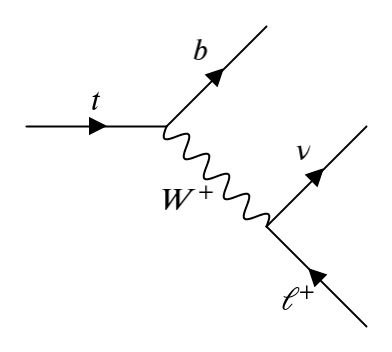
\includegraphics[width=\linewidth]{top1.png}
        \label{fig:top1}
    \end{minipage}
    \begin{minipage}{0.24\linewidth}
        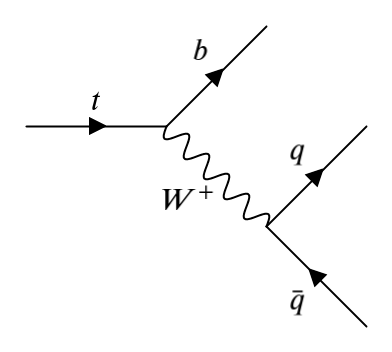
\includegraphics[width=\linewidth]{top2.png}
        \label{fig:anttop1}
    \end{minipage}
    \begin{minipage}{0.24\linewidth}
        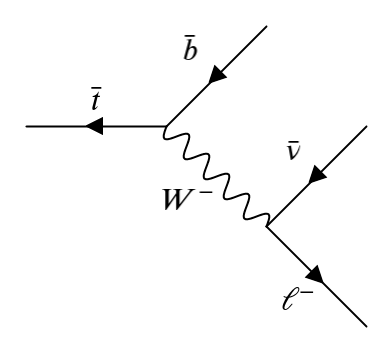
\includegraphics[width=\linewidth]{top3.png}
        \label{fig:top2}
    \end{minipage}
    \begin{minipage}{0.24\linewidth}
        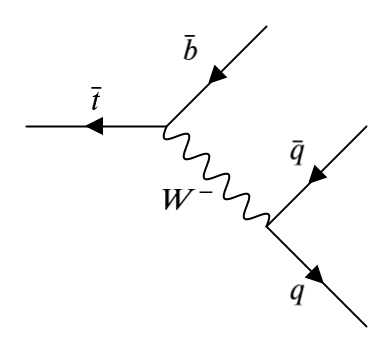
\includegraphics[width=\linewidth]{top4.png}
        \label{fig:anttop2}
    \end{minipage}
    \caption{Feynman diagrams of possible (anti-)top decays. From left to right, we see the top decay with leptonic final states, top decay with hadronic final states, anti-top decay with leptonic final states and anti-top decay with hadronic final states.}
    \label{fig:topdecay}
\end{figure}

%-------------------------------------------------------------------------%
\section{The Minimal Supersymmetric Standard Model}
The Minimum Supersymmetric Standard Model serves as an extension to the SM\footnote{The symmetry groups in the SM are contained in the MSSM, thus serving it as an extension to the SM rather than a new theory \cite{baer2006weak}} such that the particle content is duplicated once, thus keeping extra particles introduced to its minimum.  Due to the symmetry groups of the SM being contained in the MSSM, any supersymmetric transformation would yield the same quantum numbers as that of the SM \cite{aitchison2007supersymmetry}. The fermions and bosons in the SM shown in Tables \ref{tab:SMFerm} and \ref{tab:SMBos}  have \textit{superpartners}; the supersymmetric counterparts to each particle in the SM as seen in Tables \ref{tab:SUSYspart} and \ref{tab:SUSYinos}. By convention the SM particles and their superpartners are distinguished by a tilde. \\

The MSSM relies on an extended theory to the SM known as the Two-Higgs-doublt model (2HDM), in which the SM Higgs consists of the up-type Higgs ($H_u$) and the down-type Higgs ($H_d$) that contain both neutral and charged components. The SM currently only has one Higgs doublet, giving rise to four degrees of freedom that produce the Higgs boson and the gauge bosons in the SM. In the 2HDM, the number of degrees of freedom doubles to eight, leading to 5 scalar components including the physical Higgs boson. In the MSSM, the superpartners of the Higgs, the Higgsinos, are the superpartners to the 2HDM, hence the two components in Table \ref{tab:SUSYinos}.

\begin{table}[htbp]
    \centering
    \begin{tabular}{||c|c|c|c||}
    \hline
    & Gen1 & Gen2 & Gen3 \\
    \hline
    & \\[-2.7ex]
    \multirow{2}{1.4cm}{squarks} & $\Tilde{u}$ & $\Tilde{c}$ & \small$\Tilde{t}$ \\
     & $\Tilde{d}$ & $\Tilde{s}$ & $\Tilde{b}$ \\
    \hline
    
    \multirow{2}{1.4cm}{sleptons} & $\Tilde{e}$ & $\Tilde{\mu}$ & $\Tilde{\tau}$ \\
     & $\Tilde{\nu_e}$ & $\Tilde{\nu_\mu}$ & $\Tilde{\nu_\tau}$ \\
    \hline
    \end{tabular}
    \caption{The super-partners of the quarks and leptons in the SM.}
    \label{tab:SUSYspart}
\end{table}

\begin{table}[htbp]
    \centering
    \begin{tabular}{||c|c||}
    \hline 
       Gauginos  & Higgsinos \\
       \hline
        & \\[-2.5ex]
      $\Tilde{g}$, $\Tilde{B}$, $\Tilde{W}^0$, $\Tilde{W}^\pm$ & $\Tilde{H}_u$,  $\Tilde{H}_d$ \\
     \hline
    \end{tabular}
    \caption{The super-partners of the Force carriers in the SM.}
    \label{tab:SUSYinos}
\end{table}

These sparticles have simplistic names, wherein the SM matters will include an ``s" in front of the SM counterpart's name, i.e. \textit{quark} versus \textit{squark} and \textit{leptons} versus \textit{sleptons}. Furthermore, these will turn bosonic (scalar) under a SUSY transformation \cite{martin1997supersymmetry}. The gauge and scalar fields in the SM, on the other hand, will turn fermionic \cite{martin1997supersymmetry}, thus giving rise to the ``-ino" ending to the SM counterpart names, i.e. \textit{gauge bosons} versus \textit{gaugino} and \textit{Higgs} versus \textit{Higgsino}. Note that the neutral component is instead called \textit{Bino} instead of ``Zino" and \textit{Wino} has a neutral component as well.  The Higgsino in SUSY would require two independent components ($\Tilde{H}_u$ and $ \Tilde{H}_d $), unlike SM, due to Yukawa interactions being forbidden with the complex scalar field and its Hermitian conjugate \cite{aitchison2007supersymmetry}. Higgsinos would also have charged and neutral components. This alone shows that Table \ref{tab:SUSYinos} is simplified to match the number of components to Table \ref{tab:SMBos}, where in reality there are a few more extra components already due to complicated theories. \\

The MSSM, therefore, serves as an exact supersymmetric extension to the SM by introducing a \textit{minimum} number of new parameters at just one \cite{aitchison2007supersymmetry}. In other words, the number of new particles introduced is kept at a minimum to serve as a valid model beyond the SM. \\


However, this symmetry would require that these sparticles have the same mass distributions as their SM counterparts which we know not to be true simply from such particles not being observed in collider experiments. This would imply that the symmetry is broken in an unknown way, allowing these sparticles to acquire masses at a very high mass (energy) scale collider experiments cannot reach yet. MSSM also adds many more free parameters due to its constraints of introducing the minimum number of new particles. This makes things much more sophisticated and difficult to express the correct masses to the new particles exactly. \\

The gauge invariance required in the SM ``accidentally" \cite{martin1997supersymmetry} guarantees the conservation of quantum numbers known as baryon (B) and lepton (L) numbers for all interactions \cite{baer2006weak}. In MSSM, $B$ and $L$ are not necessarily conserved thus not considered as fundamental symmetries nature as there are $B$- and $L$- violating effects strongly constrained by experiment \cite{martin1997supersymmetry}. One can then introduce a globally symmetric and newly conserved quantum number \textit{R-parity} \cite{martin1997supersymmetry, baer2006weak} represented by Equation (\ref{eq:MPrec})
\begin{equation}
    P_R=(-1)^{3(B-L)+2s}
    \label{eq:MPrec}
\end{equation}
where $s$ is the spin of the particle. Different literature may simply denote $P_R$ \cite{martin1997supersymmetry} as $R$ \cite{baer2006weak}. This symmetry conveniently separates SM particles and sparticles in a way that the SM particles have $P_R=+1$ (even R-parity), whereas the sparticles all have $P_R=-1$ (odd R-parity) \cite{martin1997supersymmetry}. In MSSM, the conservation of $R$-parity comes from SUSY events as a pair-produced event \cite{aitchison2007supersymmetry}. \\

The MSSM introduces one extra particle known as the lightest supersymmetric particle (LSP) which is stable and neutral, supporting the theoretical properties of a proposed dark matter in cosmology. Analogous to dark matter, a candidate particle is introduced named as \textit{neutralino}. To be precise, there are four possible neutralinos formed by the combination of neutral higgsinos ($\Tilde{H}_u^0$ and $ \Tilde{H}_d^0 $) and neutral gauginos ($\Tilde{B}$ and $\Tilde{W}^0$), denoted as $\Tilde{N}_i$ for $i=1,2,3,4$ \cite{martin1997supersymmetry}. The hierarchy of their mass is $ m_{\Tilde{N}_1} < m_{\Tilde{N}_2} < m_{\Tilde{N}_3} < m_{\Tilde{N}_4}$, where the lightest of the four ($\Tilde{N}_1$) is the prime candidate to be the LSP unless $R$-parity is not conserved \cite{martin1997supersymmetry}. For further information regarding the generation of mass terms and their properties, the reader is referred to SUSY textbooks such as references \cite{martin1997supersymmetry} and \cite{baer2006weak}. \\

The LSP ($\Tilde{N}_1$ sometimes denoted as $\Tilde{\chi}_i^0$) is the only neutralino that cannot decay, whereas other heavier neutralinos may decay via two-body, three-body decays and so on. In collider experiments, the `detection' of the LSP would rely on searching through the missing energies of a SUSY event which is thought to be at the order of $ 2m_{\Tilde{N}_1}$ \cite{aitchison2007supersymmetry}, hence making them difficult to detect.  \\
